\documentclass{standalone}

\usepackage{xparse}
\usepackage{tikz}

\usetikzlibrary{3d}
\makeatletter
\tikzoption{canvas is xy plane at z}[]{%
  \def\tikz@plane@origin{\pgfpointxyz{0}{0}{#1}}%
  \def\tikz@plane@x{\pgfpointxyz{1}{0}{#1}}%
  \def\tikz@plane@y{\pgfpointxyz{0}{1}{#1}}%
  \tikz@canvas@is@plane
}
\makeatother


\NewDocumentCommand{\DrawCoordinateGrid}{O{} m m m m m m}{%
    \def\XGridMin{#2}
    \def\XGridMax{#3}
    \def\YGridMin{#4}
    \def\YGridMax{#5}
    \def\ZGridMin{#6}
    \def\ZGridMax{#7}
    %
    \begin{scope}[canvas is xy plane at z=0, very thin, black]
      \draw [#1] (\XGridMin,\YGridMin) grid (\XGridMax,\YGridMax);
    \end{scope}
    \begin{scope}[canvas is yz plane at x=0, very thin, black]
      \draw [#1] (\YGridMin,\ZGridMin) grid (\YGridMax,\ZGridMax);
    \end{scope}
    \begin{scope}[canvas is xz plane at y=0, very thin, black]
      \draw [#1] (\XGridMin,\ZGridMin) grid (\XGridMax,\ZGridMax);
    \end{scope}
}%

\NewDocumentCommand{\DrawCoordinateAxis}{O{} m m m m m m}{%
    \def\XAxisMin{#2}
    \def\XAxisMax{#3}
    \def\YAxisMin{#4}
    \def\YAxisMax{#5}
    \def\ZAxisMin{#6}
    \def\ZAxisMax{#7}
    %
    \begin{scope}[thin, gray, -latex]
        \draw [#1] (\XAxisMin,0,0) -- (\XAxisMax,0,0) node [below left] {$y$};
        \draw [#1] (0,\YAxisMin,0) -- (0,\YAxisMax,0) node [right] {$z$};
        \draw [#1] (0,0,\ZAxisMin) -- (0,0,\ZAxisMax) node [above] {$x$};
    \end{scope}
}%


\begin{document}
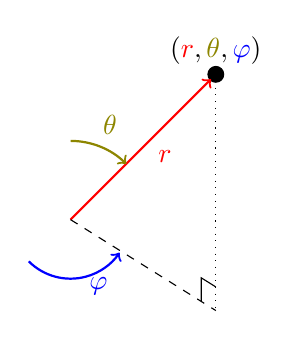
\begin{tikzpicture}[
    x={(1.0cm,0.0cm)}, y={(0.0cm,1.0cm), z={(-0.5cm,-0.1cm)}}% All grids are ok
    ]

    \DrawCoordinateGrid{0}{3.2}{0}{3.2}{0}{3.2}
    \DrawCoordinateAxis[thick, black]{0}{3.5}{0}{3.5}{0}{4}
    \draw[fill=black] (3,3,3) circle (0.1);
    \draw (3,3,3) node[anchor=south]{$(\textcolor{red}r,\textcolor{olive}\theta,\textcolor{blue}\varphi)$};
    \draw (3,0.3,3)--(2.7,0.3,2.7)--(2.7,0,2.7);
    \draw[red, thick, ->] (0,0,0) -- (2.9,2.9,2.9);
    \node at (1.2,0.8,0) {$\textcolor{red}r$};
    \draw[olive, thick, <-] ([shift=(45:1)]0,0,0) arc (45:90:1);
    \draw[olive] (0.5,1.2,0) node{$\theta$};
    \draw[thin, dotted] (3,3,3) -- (3,0,3);
    \draw[dashed] (0,0,0) -- (3,0,3);
    \draw[blue, thick, ->] ([shift=(225:0.75)]0,0,0) arc (225:326:0.75);
    \draw[blue] (1.2,0,2.2) node{$\varphi$};

\end{tikzpicture}
\end{document}